\section{Methods}
\subsection{Participants}
\subsection{Design}
This study explored the impact of various gamified elements and participant gender on performance and anxiety.
The independent variables were gamified elements, with participants randomly assigned to one of eight conditions: Avatars (A), Badges (B), Points (P), Leaderboards (L), Narrated Content (N), combinations of Points, Badges, Leaderboards, and Avatars (PBLA), Points, Badges, Leaderboards, Avatars, and Narrated Content (PBLAN), and a control group with no gamified elements.
Each participant experienced three of these conditions, ensuring that all conditions were evenly distributed across participants.
Participants underwent a series of tests in a fixed order during each round, beginning with a gamified performance test in an digital learning environment followed by  not gamified assessments for anxiety, self-efficacy, and motivation.
The performance tests utilized standard progressive matrices, adapted with gamification techniques to engage and challenge participants uniquely in each round.
The dependent variables included:
\begin{itemize}
    \item \textbf{Performance}, assessed through accuracy and response times in the gamified progressive matrices.
    \item \textbf{Anxiety}, evaluated using a standardized questionnaire immediately after the performance test.
\end{itemize}

Although self-efficacy and motivation were also assessed through subsequent questionnaires, these variables were not analyzed within the scope of this bachelor thesis.
The collected data for self-efficacy and motivation are intended for use in the doctoral dissertation of \textbf{Nadine Koch}.
This research employed a repeated-measures design, where each participant was exposed to three different gamification conditions chosen randomly.
This within-subjects approach facilitated the analysis of individual responses to each condition across the different rounds, providing insights into how variations in gamification can affect psychological states and performance.
The sequence and consistency of the testing procedure, including the series of questions asked in the gamified digital learning environment were always maintained to ensure the reliability of measurements and comparability of results across the various stages of the experiment.
\subsection{Procedure and Materials}
The study was conducted in two seperate rooms, one equipped with 5 and one with 7 iMac's. The study was displayed in full-screen mode to ensure no further distractions.
At the start participants were shown a consent form as at least some personal data was collected, gender, age and study program. Participants also had to enter a deletion code in order to request their data's deletion after the collection.
\begin{minipage}{\textwidth}
    \includegraphics[width=0.6\textwidth]{img/details.png}
    \captionof{figure}{The personal detail collection form}
    \label{fig:figureDetails}
  \end{minipage}
\subsubsection{Question items}
Afterwards the study proceeded to three iterations of 20 questions each, that are based on Progressive Matrices used by \Textcite{albuquerqueDoesGenderStereotype2017}.
Every iteration was followed by three questionnaires for anxiety, motivation and self-efficacy. Then a data submission dialog guided the participants to the next iteration.
\begin{minipage}{\textwidth}
    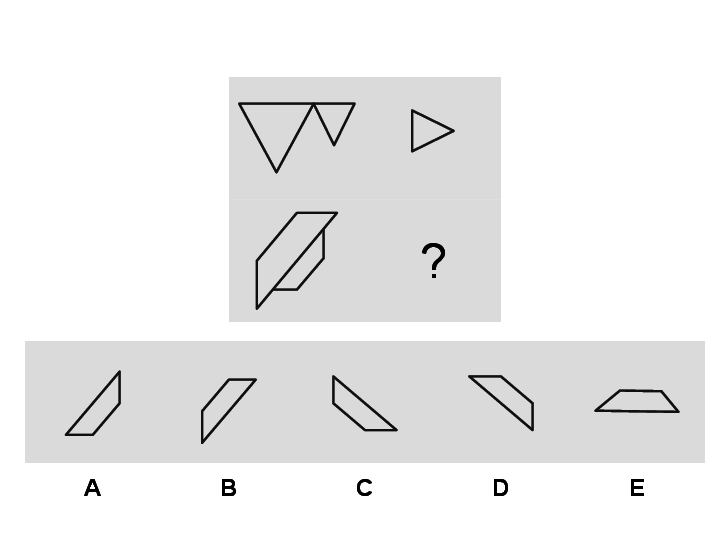
\includegraphics[width=0.6\textwidth]{img/q-17.png}
    \captionof{figure}{A standard progressive matrix, one of the tasks given to the participants}
    \label{fig:figureMatrix}
  \end{minipage}
  
To generate 60 questions out of the 20 from\textcite{albuquerqueDoesGenderStereotype2017}, the questions were slightly altered by this author.
These questions are embedded into the digital gamified learning environment.
\subsubsection{Gamified Digital Learning Environment}
The Environment used a combination of different Gamified Elements for each iteration.
\begin{minipage}{\textwidth}
    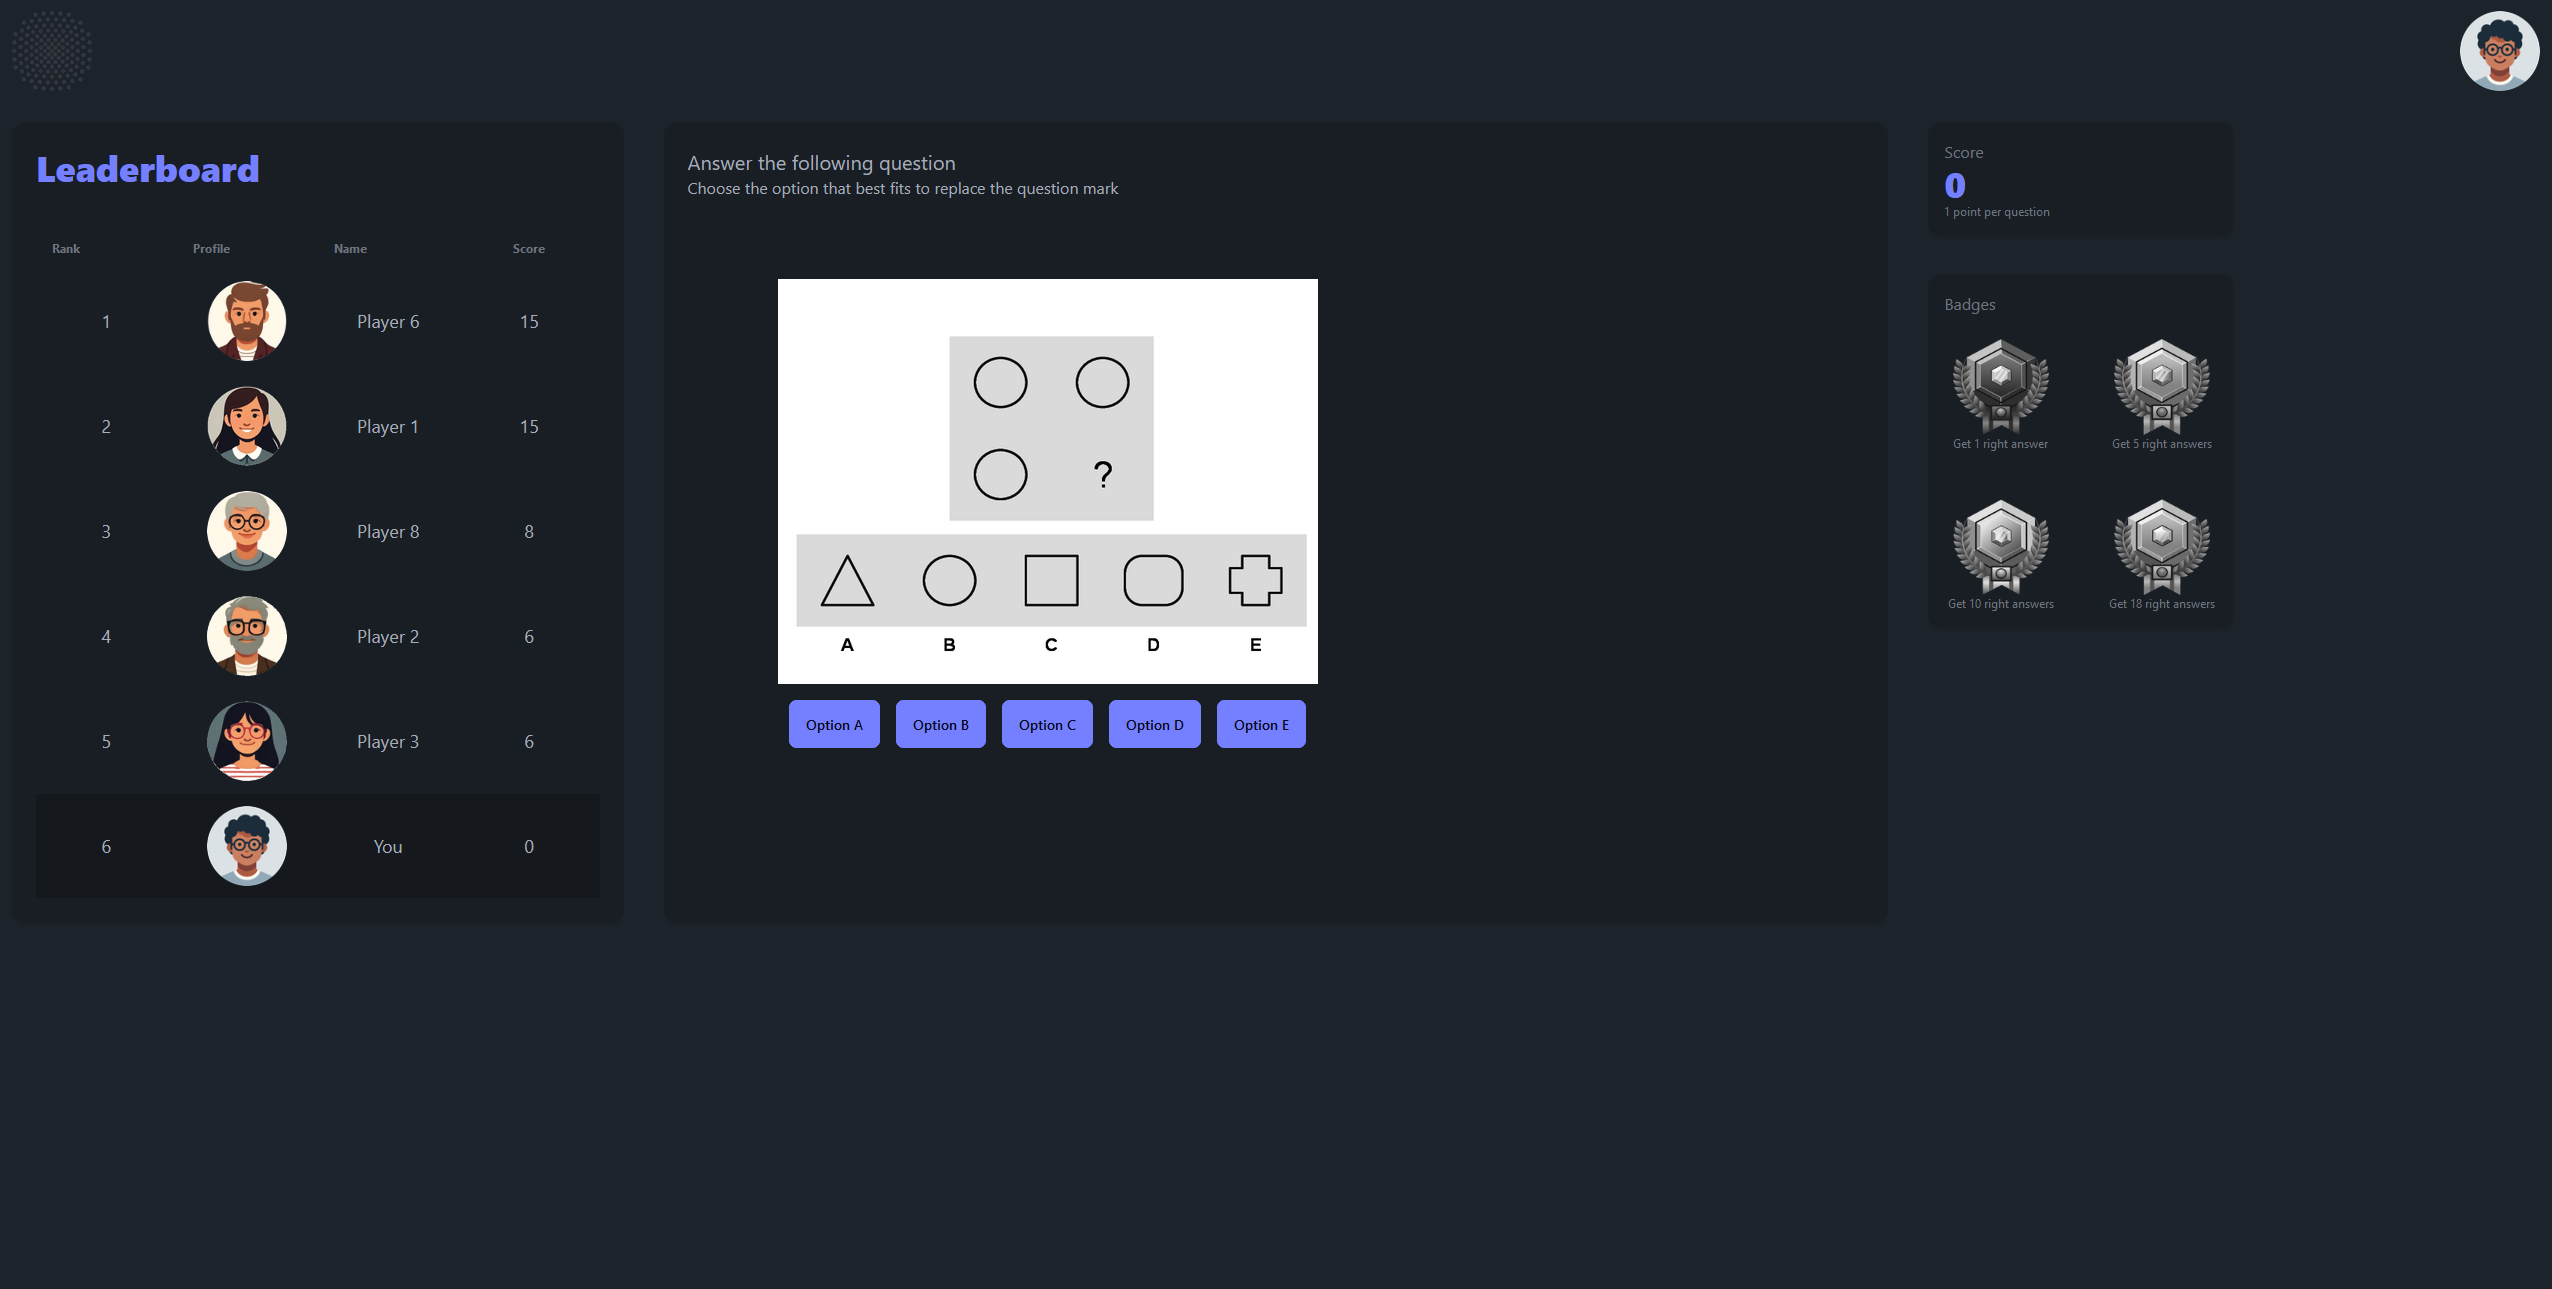
\includegraphics[width=0.6\textwidth]{img/question_screen.png}
    \captionof{figure}{The Digital Learning Environment with Points, Badges, Leaderboards and Avatars enabled.}
    \label{fig:figureScreen}
  \end{minipage}
  
\subsection{Scoring}